\chapter{腹侧前额叶皮层:基于视听内容生成目标}
这本书提出了关于灵长类动物前额叶皮层基本功能的方案。
腹侧 PF 皮层根据视觉和听觉线索生成目标,我们称之为标志,它的连接解释了为什么只有它才能做到这一点。腹侧 PF 皮层与颞下皮层的视觉区和颞上皮层的听觉区以及其他PF区有联系。它与颞叶皮层的连接提供了视觉和听觉信号,从而建立了当前的行为环境。眼眶 PF 皮层提供了选择和结果之间的联系,有时可以在单个事件的基础上学习(第4章)。在许多任务中,腹侧 PF 皮层根据具体物体和地点生成目标。然而,在涉及抽象规则和策略的任务中,腹侧PF皮层可以生成一组或几类目标以供选择或避免。鉴于腹侧PF皮层在类人猿灵长类动物中进化第2章),我们认为它在使用视觉标志和声音信息方面具有优势,可以指导近距离和远距离的觅食选择。
\section{介绍}
正如第 2 章所指出的,人们经常将灵长类动物描述为“视觉动物”。原因是中央凹在早期的单鼻科动物中进化,而三色视觉在类人猿中进化。 这些进步使这些动物及其后代能够辨别位置、颜色、形状、视觉纹理、光泽度和半透明度的微小差异。本章回顾了类人猿使用这些视觉特征来提供觅食机会线索的证据,我们称之为标志。正如第2章所解释的那样,我们所说的符号是指用作提示但不一定对应于整个对象的非空间景象和声音。
进化已经设计出许多方法来获得觅食优势。一些哺乳动物通过精心制作身体部位来开发资源,从而利用了它们的生态位。大象的长鼻子使它们能够以其他哺乳动物无法做到的方式觅食。长颈鹿的长脖子同样提供了独特的觅食机会。我们认为,类人猿反而精心设计了某些大脑结构,包括腹侧PF皮层。
\begin{figure}
	\centering
	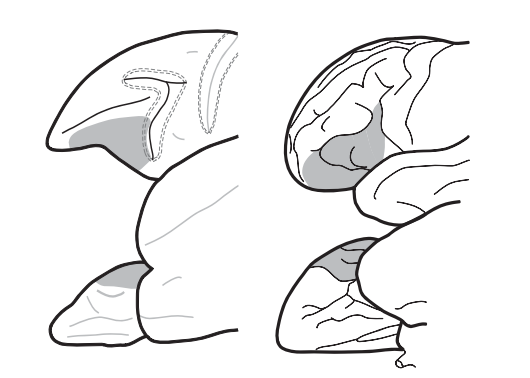
\includegraphics[width=0.7\linewidth]{image_pfc/Fig_7_1}
	\caption{猕猴(左)和人类(右)的腹侧PF皮层。格式如图1.2所示。}
	\label{fig:fig}
\end{figure}
前一章解释了背侧PF皮层生成适合当前上下文的目标,如最近事件指定的,尤其是视觉事件。它解释了视觉线索的顺序、位置和时间的重要性,以及其他特征,强调与后顶叶皮层的联系。腹侧PF皮层与下颞叶皮层和上颞叶皮层相连。因此,可见或可听的标志也指定了当前的上下文,类人猿可以单独使用或结合由顺序、位置和时间确定的上下文使用。
\section{区域}

\section{连接}

\section{视觉和听觉条件任务}

\section{视觉空间和视觉运动协会}

\section{样本匹配任务}

\section{分类}

\section{抽象规则}

\section{改变规则}

\section{抽象策略}

\subsection{结论}


